\documentclass[12pt]{article}

\usepackage{graphicx}
\usepackage{algpseudocode}
\usepackage{algorithm}
\usepackage{amsmath}
\usepackage{amssymb}
%\usepackage{subfigure}
\newcommand{\argmin}{\operatornamewithlimits{arg\ min}}
\usepackage{xcolor}
\usepackage{multirow}
\usepackage{multicol}
\usepackage{makecell}
\usepackage{caption}
\usepackage{subcaption}
\usepackage{soul}

\begin{document}

\section{Training Effect}

\begin{figure}[h]
	\begin{center}
		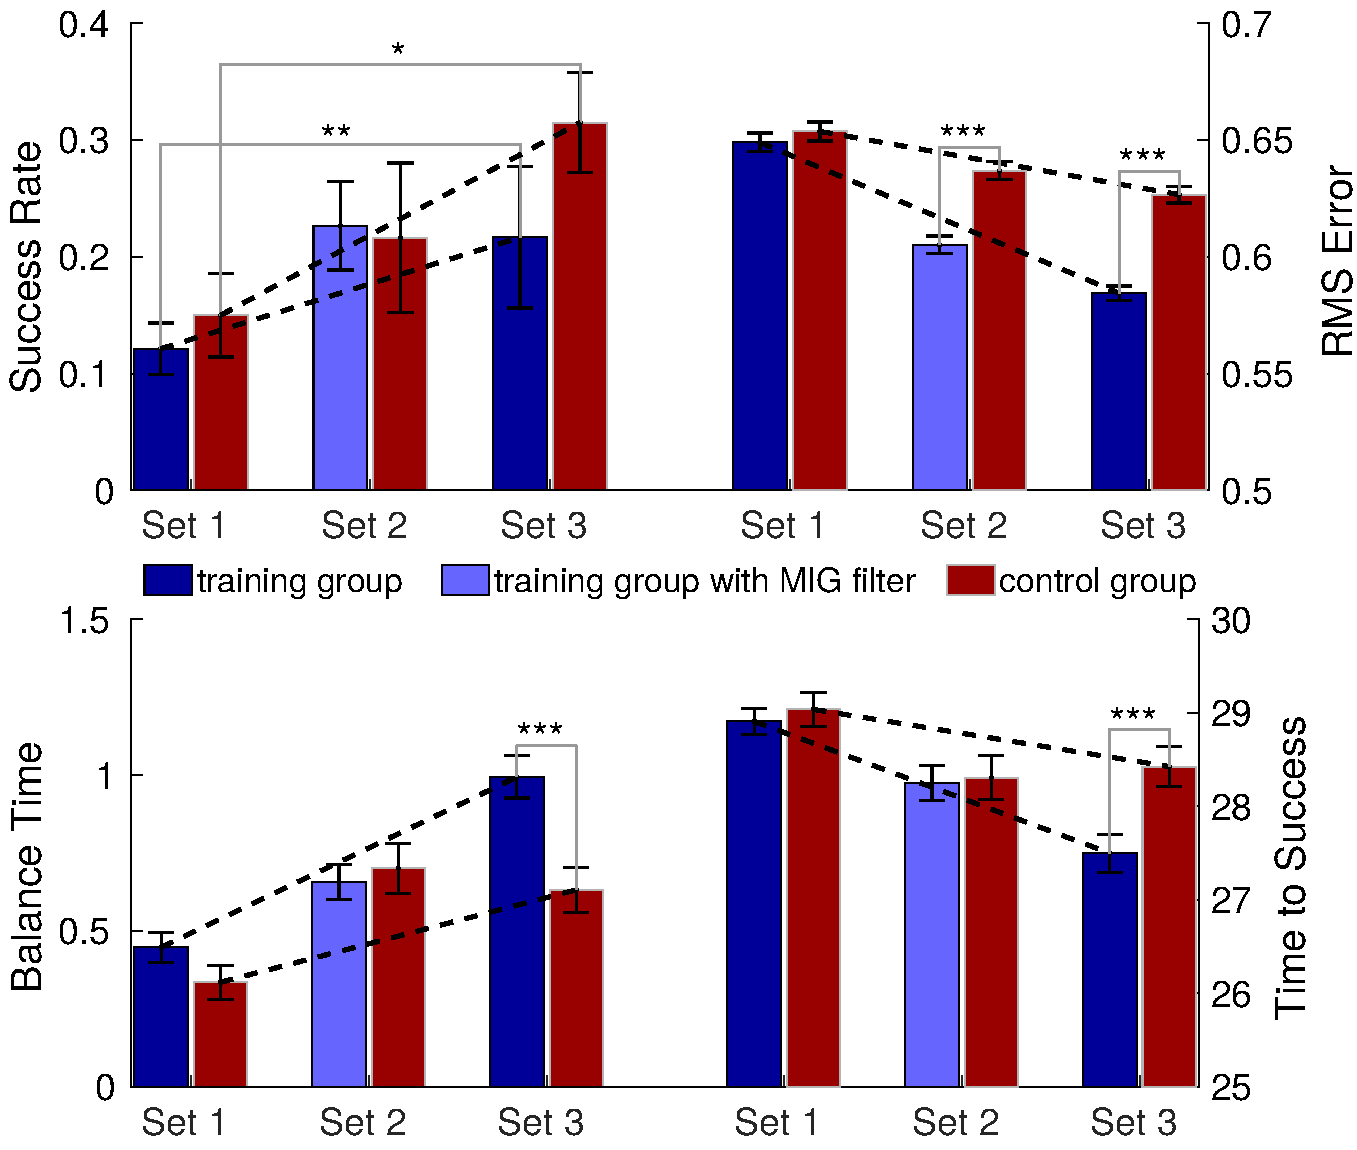
\includegraphics[width=\columnwidth]{training.pdf}
	\end{center}
	\caption{There was a training effect from training with the filter-based feedback compared to training with no feedback. The RMS error, balance time, and time to success of the training group in the final set was significantly better than that of the control group. It is also worth noting that as expected, pairwise comparisons of the two groups in set 1 show that there was not a significant difference in their baseline performance measurements. Moreover, set was consistently the most significant factor in performance improvements from set 1 to set 3, showing that both groups (training and control) improved significantly over time. Finally note that error bars indicate standard error and significance is indicated by $^*p<0.05$, $^{**}p<0.01$, $^{***}p<0.001$.}
	\label{fig: training}
\end{figure}

The main result we were looking for in the study was whether providing filter-based feedback through forceful interaction would improve learning. And indeed, we observed a significant training effect from training with filter-based feedback compared to training with no feedback for an equivalent duration of time, as visible in Fig.~\ref{fig: training}. \textit{Post hoc} analysis confirmed that both groups started the experiment at comparable skill levels and although training time was the main factor impacting improvement in performance (both groups improved over time), the training group improved significantly more than the control. Detailed statistical analysis is described below. 

A two-factor repeated measures ANOVA was used to assess the effects of the group (between-subjects) and set (within-subjects) on all performance measures listed in Section~\ref{metrics} of Chapter~\ref{chapter: methods}. The training group and control group were evaluated based on set 1 and set 3 only. Set 2 was left out of the ANOVA, so that effects of the assistance itself would not be measured in the analysis. Additionaly, pairwise comparisons were made between set 1 for both groups, between set 3 for both groups, and between set 1 and set 3 within each group using a paired 2 sample t-test. 

Firstly, we confirmed that there was on average no difference in skill at the onset of the experiment. Pairwise comparisons within each of the four measures (success rate, RMS error, balance time, and time to success) showed that in set 1 there was not a significant difference between the training group and control group. For instance, the main effect of group in set 1 on the RMS error was not significant ($F(1,26)=1.615, p = 0.215$)---there was not a significant difference between the training group ($mean =0.612, SD =0.088$) and the control group ($mean = 0.639 , SD=0.067$) in set 1. The same was true for the three other metrics. According to 2-sample t-tests, the differences between the two groups were also not significant across all 4 metrics ($p>0.01$).

Secondly, we found that time had the most significant impact on learning. The factorial ANOVA revealed that for success rate the main effect of set yielded an F ratio of $F(1,50)=7.555,\ p=0.008$, meaning that users were more successful in set 3 ($mean =0.280 , SD = 0.223$) than in set 1 ($mean = 0.140,\ SD = 0.100$) regardless of the type of practice in set 2. Similarily, the RMS error showed that the main effect of set yielded an F ratio of $F(1,26) = 41.551, p<0.001$, indicating a significant difference between set 1 ($mean =0.651, SD =0.085$) and set 3 ($mean =0.599, SD =0.072$). The main effect for set on the balance time yielded an F ratio of $F(1,26)=15.328,\ p<0.001$, indicating a significant difference between the balance time in set 1 ($mean = 0.408, SD = 1.053$) and set 3 ($mean = 0.866, SD = 1.476$). The main effect of set on time to success was also significant ($F(1,26)=18.992,\ p<0.001$), with set 3 ($mean = 27.830, SD = 4.433$) outperforming set 1 ($mean = 28.955,SD =3.175$). Set had a significant effect on increases across all metrics, indicating that participants were continuously improving with time regardless of the feedback that was provided. 

Thirdly, we observed that there was more improvement among members of the training group than control. When training group and control group were compared in set 3 using 2-sample t-tests, the training group performed better. The set 3 balance time of the control group ($mean =0.632, SD = 1.261$) was significantly less ($t(728)=3.643,p<0.001$) than the balance time of the training group ($mean = 0.994 , SD = 1.568$). The time to success was also significantly better ($t(738)=3.110, p=0.002$) in set 3 of the training group ($mean = 27.500, SD = 4.744$) compared to set 3 of the control group ($mean =28.43, SD = 3.74$). The same was true for the RMS error ($t(699)=-8.919,p<0.001$)---the RMS error of the training group in set 3 ($mean = 0.58, SD = 0.003$) was lower than the RMS error of the control ($mean = 0.63, SD = 0.004$). The RMS error, balance time, and time to success of the training group in the final set was significantly better than that of the control, while the difference for success rate was not statistically significant. 

Moreover, the RMS error showed that there was a significant interaction effect between group and set ($F(1,26)=5.099, p=0.0326$). This is indicated in Fig.~\ref{fig: training} by the two groups having similar means in set 1 but significantly different means in set 3, implying that the training had a greater impact on set 3 performance than the unassisted practice of the control group. For the other measures, the interaction effects were statistically insignificant---there was no significant interaction effect of group and set on balance time ($F(1,26)=1.048,\ p=0.315$), time to success ($F(1,26)=1.512,\ p=0.22983$) or success rate ($F(1,50)=0.111,\ p=0.740$). There was also no signifcant effect of group on any of the metrics: success rate ($F(1,50)=0.981,\ p=0.327$), balance time ($F(1,26)=1.562,\ p=0.223$), time to success ($F(1,26) = 1.114,\ p=0.301$), or RMS error ($F(1,26) = 1.824 ,\ p=0.189$). In summary, although there was not a significant effect of group on any of the  metrics, the RMS  error  showed  that there  was  a  significant  interaction  effect between  group  and set.  

% Although the change in success rate from set 1 to set 3 was significant for both the control group ($t(9)=3.152,\ p = 0.012$) and the experimental group ($t(17)=3.127,\ p=0.006$), the effect size of the training group ($d=0.94$) from set 1 to set 3 was larger than the effect size of the control group ($d=0.77$). (XXX why report this only for success rate?) 

 % Note that the control group continued to improve their success rate with each set, possibly because their interaction with the robot did not change between sets as it did for the training group. 


\begin{figure}[h]
	\begin{center} 
	\begin{multicols}{2}
		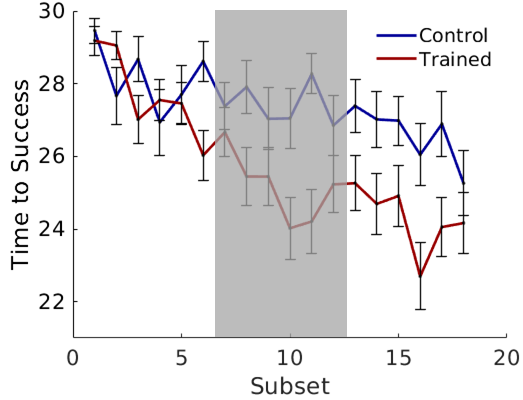
\includegraphics[width=0.85\columnwidth]{tts_plateau.png}
		\caption*{}
		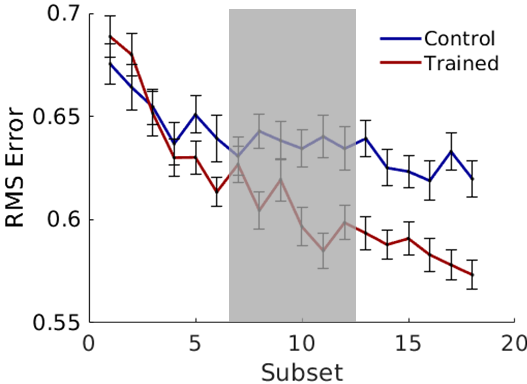
\includegraphics[width=0.9\columnwidth]{err_plateau.png}
		\caption*{}
	\end{multicols}
	\end{center}
	\vspace{-1.2cm}
	\caption{Grey band covers subsets included in set 2 (the set, where the training group received feedback). Note that training and control groups showed similar improvement during set 1, while the training group showed faster improvement during set 2. Particularly with respect to the RMS error, the control group's improvement slows down drastically during set 2, while the training group keeps improving.}
	\label{fig: plateau}
\end{figure}


Finally, in order to assess how subject performance evolved over time, the baseline and post-training sets were analyzed using subsets containing five individual trials, rather than the sets of thirty trials used for the analysis above. As such, there were 6 subsets in each set as shown in Fig.~\ref{fig: plateau}. We can see that the training and control groups diverage in performance during the subsets of set 2. Particularly with respect to the RMS error, the control group plateaus in improvement while the training group keeps improving. These results support the hypothesis that subjects experience accelerated learning while receiving feedback through filter-based forceful interaction. 

\end{document}